\documentclass{article}
\usepackage{stocktonmacros} % Personal macros, import package
\setlist[itemize]{noitemsep, topsep=0pt} % Must keep within the same document as \begin{document}

\begin{document}

%\maketitle
%%
%\newpage
%%
%\tableofcontents
%%%
%\newpage
%%%
%\import{Lectures/}{Partial Differential Equations - An Introduction}
%\import{Lectures/}{Heat, Wave Equation}
%\import{Lectures/}{Approximating Functions with Other Functions}
%\import{Lectures/}{Heat Equation}
%\import{Lectures/}{Wave Equation}
%\import{Lectures/}{Boundary Conditions}
%\import{Lectures/}{Laplace's Equation}
%\import{Lectures/}{Polar Coordinates}
%\import{Lectures/}{Complex Analysis, Fourier Transform}
%\import{Lectures/}{Transport Equation}
%\import{Lectures/}{Image Processing}
%\import{Lectures/}{Exam 2 Review}
\import{Lectures/}{Conservation Laws}
%______________________________________________________________________________%
\newpage
% Conservation Law?
\subsection{Traffic Flow}
\topic{April 11, 2022}
Conservation of Cars

Traffic in - Traffic out = Accumulated traffic

\begin{center}
  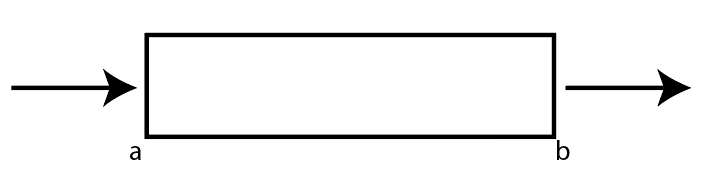
\includegraphics{Conservation Laws - Traffic Flow 1}
\end{center}

Let $\rho(x, t)$ be the density and $q(x, t)$ is the flux.
%
\begin{align}
  \frac{d}{dt} \int^b_a \rho(x, t)\ \text dx
  & = q(a, t) - q(b, t)\\
  & = -\int^b_a q_x (x, t)\ \text dx\\
  \int^b_a (\rho_t + q_x)\ \text dx & = 0\\
  \rho_t + q_x & = 0
\end{align}

Here, $u$ is car velocity:
%
\begin{align}
  q & = pu
\end{align}

Now,
%
\begin{align}
  \rho_t + [\rho u]_x & = 0
\end{align}

Both $\rho$ and $u$ are a function of $x$, therefore there is a
product rule that comes into play.
%
\begin{align}
  \rho_t + [c(\rho)]\rho_x & = 0
\end{align}

We have yet to determine $c$. So far, this equation is similar to the Transport
Equation, where we use $c$ to find the speed of the equation.

$c(\rho)$ will give the speed of the characteristic.

In general, the car velocity should be a decreasing function of $\rho$.

When $\rho = 0$, the car moves the fastest $= u_{\text{max}}$

When $\rho = \rho_{\text{max}} \Rightarrow u = 0$

The simplest relationship which satisfies these is:
%
\begin{align}
  u(\rho) & = u_{\text{max}}\left(1 - \frac{\rho}{\rho_{\text{max}}}\right)
\end{align}

This tells me,
%
\begin{align}
  q(\rho)
  & = u_{\text{max}} \rho\left( 1 - \frac{\rho}{\rho_{\text{max}}}\right)\\
  & = u_{\text{max}} \rho - \frac{u_{\text{max}}}{\rho_{\text{max}}} \rho^2
\end{align}

Hit maximum velocity at $\frac{\rho_{text{max}}}{2}$
%
\begin{align}
  q_x
  & = u_{\text{max}} \rho_x - 2 \frac{u_{\max}}{\rho_{\max}} \rho \rho_x\\
  & = u_{\max} \left[ 1 - \frac{2}{\rho_{\max}} \rho \right] \rho_x
\end{align}

Here, this shows our critical point is at $\frac{\rho_{\max}}{2}$. Let us
redefine this equation as $c(\rho) \rho_x$.
%
\begin{align}
  \rho_t + u_{\max} \left( 1 - \frac{2\rho}{\rho_{\max}}\right) \rho_x & = 0
\end{align}

\ex When a red light turns green.
%
\begin{align}
  \rho(x, t) & =
  \begin{cases}
    \rho_{\max} & x < 0\\
    0 & x > 0
  \end{cases}
\end{align}

Recall, the speed of our characteristic:
%
\begin{align}
  c(\rho) & = u_{\max} \left(1 - \frac{2 \rho}{\rho_{\max}}\right)
\end{align}

The slope of our characteristic is:
%
\begin{align}
  & = \frac{1}{u_{\max} \left(1 - \frac{2 \rho}{\rho_{\max}}\right)}
\end{align}

When we have $\rho = \rho_{\max}$, our slope is $- \frac{1}{u_{\max}}$.

When we have $\rho = 0$, our slope is $\frac{1}{u_{\max}}$.
%
\begin{align}
  \rho(x, t) & =
  \begin{cases}
    \rho_{\max} & x < - u_{\max} t\\
    \frac{\rho_{\max}}{2} \left(1 - \frac{x}{u_{\max}t}\right)
    & -u_{\max} t < x < u_{\max} t\\
    0 & x > u_{\max} t
  \end{cases}
\end{align}

\ex When the light turns red, hit bumper-to-bumper traffic.

For $x < 0$, we have $\rho(x, 0) = \rho_0$.

For $x > 0$, we have $\rho(x, 0) = \rho_{\max}$.

Here, let us write:
%
\begin{align}
  u_t + [f(u)]_x & = 0\\
  \xi^\prime(\aleph) & = \frac{f(u_L) - f(u_R)}{u_L - u_R}
\end{align}

Our $q$ is:
%
\begin{align}
  q(\rho) = u_{\max} \rho\left(1 - \frac{\rho}{\rho_{\max}}\right)
\end{align}

If we consider our graph, a shock will form and we will have:
%
\begin{align}
  \xi^\prime(t) & = \frac{q(\rho_L) - q(\rho_R)}{\rho_L - \rho_R}\\
  & = \frac{u_{\max} \rho_0 \left( 1 - \frac{\rho_0}{\rho_{\max}
  - 0}\right)}{\rho_0 - \rho_{\max}} < 0
\end{align}

\topic{April 13, 2022}

\ex Green light turns red, then green

\begin{center}
  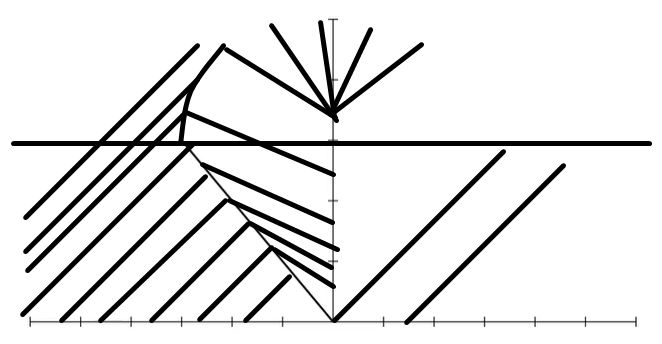
\includegraphics{Traffic Light - Turning Red}
\end{center}

\subsection{Method of Characteristics}

We will look at agns? of the form:
%
\begin{align}
  a(x, t) u_x + b(x, t) u_t + c(x, t) u & = 0\\
  u(x, 0) & = f(x)
\end{align}

Let:
%
\begin{itemize}
  \item $x(t)$ : Moving observer <- Location of observer
  \item $u(x, t)$ : function of $x$ and $t$
\end{itemize}

How does $u$ change from the observer's perspective?

How does a point in front of one move?

Find $\frac{du}{dt}$:
%
\begin{align}
  \frac{du(x(t), t)}{dt} & = \frac{du}{dt} + \frac{\p u}{\p x} \frac{dx}{dt}\\
  & = u_t + u_x \frac{dx}{dt}
\end{align}

\ex Transport Equation
%
\begin{align}
  u_t + cu_x & = 0\\
  \frac{dx}{dt} & = c\\
  \frac{du}{dt} & = 0
\end{align}

The observer is moving at speed $c$ and $u$ is not changing.

Let us consider the following:
%
\begin{align}
  u(x, 0) & = f(x)\\
  x(0) & = x_0\\
  u(0) & = u_0
\end{align}

Now, let us consider:
%
\begin{align}
  \frac{du}{dt} & = u_t + \frac{dx}{dt} u_x
\end{align}
\begin{align}
  \frac{dx}{dt} & = c\\
  x & = ct + k\\
  x & = ct + x_0\\
\end{align}
\begin{align}
  \frac{du}{dt} & = 0\\
  u & = u_0\\ & = u(x_0, 0)\\ & = f(x_0)\\ & = f(x - ct)
\end{align}

\note
%
\begin{align}
  u_t + cu_x & = 0\\
  \left< 1, c \right> \cdot \left< u_t, u_x \right> & = 0\\
  \left< 1, c \right> \cdot \left< \grad \right> & = 0
\end{align}

Here, we found the directional derivative.

\ex $u_t + cu_x = 1$ and $u(x, 0) = \sin x$
%
\begin{align}
  \frac{dx}{dt} = c & \Rightarrow x = ct + x_0\\
  \frac{du}{dt} = 1 & \Rightarrow u = t + B\\
  u(x_0, t) & = u_0\\
  & = t + u_0 = t + u(x_0, 0)\\
  & = t + \sin x_0\\
  & = t + \sin(x - ct)
\end{align}

\ex $u_t + cu_x + au = 0$, $u(x, 0) = f(x)$
%
\begin{align}
  u_t + cu_x & = -au\\
  \left< 1, c \right> \cdot \left< u_t, u_x \right> & = -au
\end{align}

If $a > 0$, directional derivative $= -au \Rightarrow$ decay
%
\begin{align}
  \frac{dx}{dt} = c & \Rightarrow x = ct + x_0
\end{align}

The following is an exponential decay (Refer to Differential Equation):
%
\begin{align}
  \frac{du}{dt} & = -au\\
  u & = De^{-at} = u_0 e^{-at}
\end{align}

When we plug in $t = 0$, we should get $f(x)$:
%
\begin{align}
  u & = f(x_0) e^{-at}\\
  & = f(x - ct) e^{-at}
\end{align}

\ex $u_t + xu_x = 0$, $u(x, 0) = f(x)$
%
\begin{align}
  \frac{dx}{dt} = x & \Rightarrow x = x_0 e^t\\
  \frac{du}{dt} = 0 & \Rightarrow u = u_0 = f(x_0) = \left(\frac{x}{e^t}\right)
  = f(xe^{-t})
\end{align}

\topic{April 18, 2022}
%
\begin{align}
  \frac{du}{dt} & = \frac{dx}{dt} u_x + u_t
\end{align}

We can also introduce a new variable,
%
\begin{align}
  a(x, t) u_x + b(x, t) u_t + c(x, t) u & = 0\\
  \frac{dx}{ds} & = a(x, t)
\end{align}

\begin{multicols}{2}
  \begin{align}
    \frac{dx}{ds} & = a(x, t)\\
    \frac{dt}{ds} & = b(x, t)
  \end{align}

  \begin{align}
    \frac{dy}{ds} & = -c(x, t) u\\
    \frac{du}{ds} & = \frac{dx}{ds} u_x + \frac{dt}{ds} u_t
  \end{align}
\end{multicols}

\begin{center}
  \import{Snippets/}{tree_uxts}
\end{center}

\ex $xu_x + u_t + tu = 0 \Rightarrow xu_x + u_t = -tu$
%
\begin{align}
  \frac{dx}{ds} & = x \Rightarrow x = ce^s = x_0 e^s = x_0 e^t\\
  \frac{dt}{ds} & = 1 \Rightarrow t = s + t_0 = s\\
  \frac{du}{ds} & = -tu = -su \Rightarrow u = f\left(xe^{-t}\right)
  e^{-\frac{1}{2}t^2}
\end{align}

To find the third differential, we did separation of variables:
%
\begin{align}
  \int \frac{1}{u} du & = \int -s ds\\
  \ln |u| & = - \frac{1}{2} s^2 + c\\
  u & = e^{- \frac{1}{2} s^2 + c}\\
  u & = ce^{- \frac{1}{2} s^2}\\
  u & = u_0 e^{-\frac{1}{2} t^2}\\
  u & = f(x_0) e^{-\frac{1}{2}t^2}\\
  u & = f\left(xe^{-t}\right)e^{-\frac{1}{2}t^2}
\end{align}

Because $u(x 0) = f(x)$ and $x_0 = \frac{x}{e^t} = xe^{-t}$

\ex $2xtu_x + u_t = u$, $u(x, 0) = x$

Because $\frac{dt}{ds} = 1$, we do not consider $s$.
%
\begin{align}
  \frac{dx}{dt} & = 2xt \Rightarrow x = x_0 e^{t^2}\\
  \frac{du}{dt} & = u \Rightarrow u = u_0 e^t = f(x_0) e^t = f(xe^{-t^2})e^t
  = xe^{-t^2} e^t
\end{align}

Recall $u_0 = f(x)$.

Here, we found $\frac{dx}{dt}$ through separation of variables:
%
\begin{align}
  \frac{dx}{dt} & = 2xt\\
  \int \frac{1}{x} & = \int 2t dt\\
  \ln |x| & = t^2 + c\\
  x & = ce^{t^2}\\
  x & = x_0 e^{t^2}
\end{align}

\ex $u^2 \frac{du}{dx} + \frac{du}{dt} = 0$, $u(x, 0) = \sqrt x$.
%
\begin{align}
  \frac{dx}{dt} & = u^2 \Rightarrow x = u^2 t + c = u^2 t + x_0
  \Rightarrow x_0 = x - u^2 t\\
  \frac{du}{dt} & = 0 \Rightarrow u = u_0 = f(x_0) = f(x - u^2 t)
  = \sqrt{x - u^2 t} = \sqrt{\frac{x}{1 + t}}
\end{align}

Here, we solve for $u$ as:
%
\begin{align}
  u & = \sqrt{x - u^2 t}\\
  u^2 & = x - u^2 t\\
  u^2(1 + t) & = x\\
  u^2 & = \frac{x}{1 + t}\\
  u & = \sqrt{\frac{x}{1 + t}}
\end{align}

\ex $e^{t^2} u_t + tu_x = 0$, $u(x, 0) = f(x)$.

Here, let us divide out our term in front of
$u_t$ to get $u_t + te^{-t^2}u_x = 0$,
%
\begin{align}
  \frac{dx}{dt} & = te^{-t^2} \Rightarrow x = \\
  \frac{du}{dt} & = 0 \Rightarrow u = u_0 = f(x_0)
  = f(x + \frac{1}{2}e^{-t^2} - \frac{1}{2})
\end{align}

To solve for $x$,
%
\begin{align}
  x & = \int te^{-t^2}\\
  & = -\frac{1}{2} \int e^w \text dw\\
  & = -\frac{1}{2} e^w + c\\
  & = -\frac{1}{2} e^{-t^2} + C
\end{align}

Here, we want our term to zero out:
%
\begin{align}
  x_0 & = - \frac{1}{2} + c \Rightarrow c = x_0 + \frac{1}{2}\\
  x & = -\frac{1}{2} e^{t^2} + x_0 + \frac{1}{2}\\
  x_0 & = x + \frac{1}{2} e^{-t^2} - \frac{1}{2}
\end{align}

\ex $u_t + tu_x = u^2$, $u(x, 0) = f(x)$
%
\begin{align}
  \frac{dx}{dt} & = t \Rightarrow x = \frac{1}{2} t^2 + c
  = \frac{1}{2} t^2 + x_0 \Rightarrow x_0 = x - \frac{1}{2} t^2\\
  \frac{du}{dt} & = u^2 \Rightarrow u =
\end{align}

Here, to solve the second term,
%
\begin{align}
  \frac{du}{dt} & = u^2\\
  \int \frac{1}{u^2} \text du & = \int \text dt\\
  -\frac{1}{u} & = t + c\\
  \frac{1}{u} & = -t + c\\
  u & = \frac{1}{c - t}\\
  & = \frac{1}{\frac{1}{u_0} - t}\\
  & = \frac{u_0}{1 - u_0 t}\\
  & = \frac{f(x_0)}{1 - f(x_0)t}\\
  & = \frac{f\left(x - \frac{1}{2}t^2\right)}
  {1 - f\left(x - \frac{1}{2}t^2\right)t}
\end{align}

\topic{April 20, 2022}

\ex $tu_x - xu_t = u$ \quad $u(x, 0) = f(x)$
\begin{align}
  \frac{dx}{ds} & = t\\
  \frac{dt}{ds} & = -x\\
  \frac{du}{ds} & = u
\end{align}

Here, the issue with this format is that the first two terms have three
variables. We must find $x_0$ and to get $x_0$, we must get to $x$. To solve
this, we will look at parametric equations. Let us combine the first two lines to get:
%
\begin{align}
  \frac{dx}{dt} & = - \frac{t}{x}
\end{align}

From here, we can solve this via separation of variables
%
\begin{align}
  \int x \text dx & = \int - t \text dt\\
  \frac{1}{2} x^2 & = -\frac{1}{2} t^2 + C\\
  x^2 & = - t^2 + C\\
  x^2 + t^2 & = C\\
  x^2 + t^2 & = x^2_0
\end{align}

Now, to solve for our third term, we would get an exponential via separation of variables:
%
\begin{align}
  \frac{du}{ds} & = u \Rightarrow u = u_0 e^s
\end{align}

Here, if we want to find $t$ for $s$, we write:
%
\begin{align}
  \frac{dx}{ds} & = t \Rightarrow \frac{d^2x}{ds^2} = \frac{dt}{ds} = -x
  \Rightarrow x(s) = a \cos s + b \sin s\\
  & \Rightarrow x(0) = x_0 \rightarrow a = x_0\\
  \frac{dt}{ds} & = -x \Rightarrow \frac{d^2t}{ds^2} = -\frac{dx}{ds} = -t
  \Rightarrow t(s) = b \cos s - a \sin s\\
  & \Rightarrow t(0) = 0 \rightarrow b = 0
\end{align}

Since want to start $t$ at $0$, $\sin$ would belong to $t$.

Now, we know the following:
%
\begin{align}
  x & = x_0 \cos s\\
  t & = -x_0 \sin s\\
  \frac{t}{x} & = - \tan s
\end{align}

So, to go back to $\frac{du}{ds}$,
%
\begin{align}
  \frac{du}{ds} & = u \Rightarrow u = u_0 e^s
  = f(x_0) e^{\arctan \frac{-t}{x}}\\
  & = f\left( \sqrt{x^2 + t^2} \right) e^{\arctan \frac{-t}{x}}
\end{align}

\ex $xu_x + tu_t = 2u$ \quad $u(x_0, 1) = f(x)$
\begin{align}
  \frac{dx}{ds} & = x \Rightarrow_1 x = x_0 e^s \Rightarrow_4 x_0
  = \frac{x}{e^s} = \frac{x}{t}\\
  \frac{dt}{ds} & = t \Rightarrow_2 t = t_0 e^s = e^s\\
  \frac{du}{ds} & = 2u \Rightarrow_3 u = u_0 e^{2s}
  \Rightarrow_5 u = f(x_0) e^{2s} = f\left(\frac{x}{t}\right)(e^s)^2
  = f\left(\frac{x}{t}\right)t^2
\end{align}

\ex $u_t + tu_x = 0$, $u(x, 0) = f(x)$
%
\begin{align}
  \frac{dx}{dt} & = t \Rightarrow_1 x = \frac{1}{2}t^2 + x_0\\
  \frac{du}{dt} & = 0 \Rightarrow u = u_0 = f(x_0) = f\left(x - \frac{1}{2} t^2\right)
\end{align}

\ex $u_t + tu_x = xt$, $u(x, 0) = f(x)$
%
\begin{align}
  \frac{dx}{dt} & = t \Rightarrow_1 x = \frac{1}{2} t^2 + x_0\\
  \frac{du}{dt} & = xt = t\left(\frac{1}{2}t^2 + x_0\right)
  = \frac{1}{2} t^3 + x_0 t\\
  & \Rightarrow_2 u = \frac{1}{8} t^4 + \frac{1}{2} x_0 t^2 + u_0
  = \frac{1}{8} t^4 + \frac{1}{2} \left(x - \frac{1}{2} t^2\right)t^2 +
  f\left(x - \frac{1}{2} t^2 \right)
\end{align}

\ex $u_t + xu_x = x$, $u(x, 0) = f(x)$
%
\begin{align}
  \frac{dx}{dt} & = x \Rightarrow_1 x_0 e^t\\
  \frac{du}{dt} & = x =_2 x_0e^t \Rightarrow u = x_0e^t + C
  = x_0 e^t + u_0 - x_0 = x + f(xe^{-t}) - xe^{-t}
\end{align}

\ex $xu_x + u_t = t$, $u(x, 0) = x^2$
%
\begin{align}
  \frac{dx}{dt} & = x \Rightarrow_1 x = x_0 e^t\\
  \frac{du}{dt} & = t \Rightarrow_2 u = \frac{1}{2} t^2 + u_0
  = \frac{1}{2}t^2 + f\left(xe^{-t}\right)
  = \frac{1}{2}t^2 + \left(xe^{-t}\right)^2
\end{align}

\ex $xu_t - 2xtu_x = 2tu$, $u(x, 0) = f(x)$

Let us rewrite our equation as $u_t - 2tu_x = \frac{2tu}{x}$
%
\begin{align}
  \frac{dx}{dt} & = -2t \Rightarrow_1 x = -t^2 + x_0\\
  \frac{du}{dt} & = \frac{2tu}{x} =_2 \frac{2tu}{x_0 - t^2}
\end{align}

For the second term, we would have to separate:
%
\begin{align}
  \int \frac{1}{u} \text du & = \int \frac{2t}{x_0 - t^2} \text dt\\
  \ln |u| & = \int \frac{2t}{x_0 - t^2} \text dt
\end{align}

Here, our $w = x_0 t^2$ and $dw = -2t dt$
%
\begin{align}
  \ln |u| & = - \ln |x_0 - t^2| + C\\
  u & = ce^{-\ln|x_0 - t^2|}\\
  u & = ce^{\ln|x_0 - t^2|^{-1}}\\
  u & = \frac{c}{x_0 - t^2}
\end{align}

Here, we know $x_0$ and we can find $c$ since plugging in $0$ should give us
$u_0$:
%
\begin{align}
  & = \frac{x_0 u_0}{x_0 - t^2}\\
  u & = \frac{(x + t^2) f(x_0 + t^2)}{x}
\end{align}
\end{document}
